\section{研究问题}

\begin{frame}{开场}
  各位老师、各位同学，大家好。

  \vspace{0.6em}
  我今天汇报的题目是《数字化转型的投资结构优化效应》，这是我和我的导师王倩教授合作完成的一篇文章。

  \vspace{0.8em}
  接下来的汇报，我打算沿着这样一个思路展开：
  \begin{enumerate}
    \item 先跟大家聊聊我们为什么要关心这个问题；
    \item 然后介绍我们是怎么用模型把故事讲清楚的；
    \item 再看看数据上能不能找到支持这个故事的证据；
    \item 最后讨论这些发现意味着什么。
  \end{enumerate}
\end{frame}

\begin{frame}{一个持续了近三十年的宏观趋势}
  \begin{figure}
    \centering
    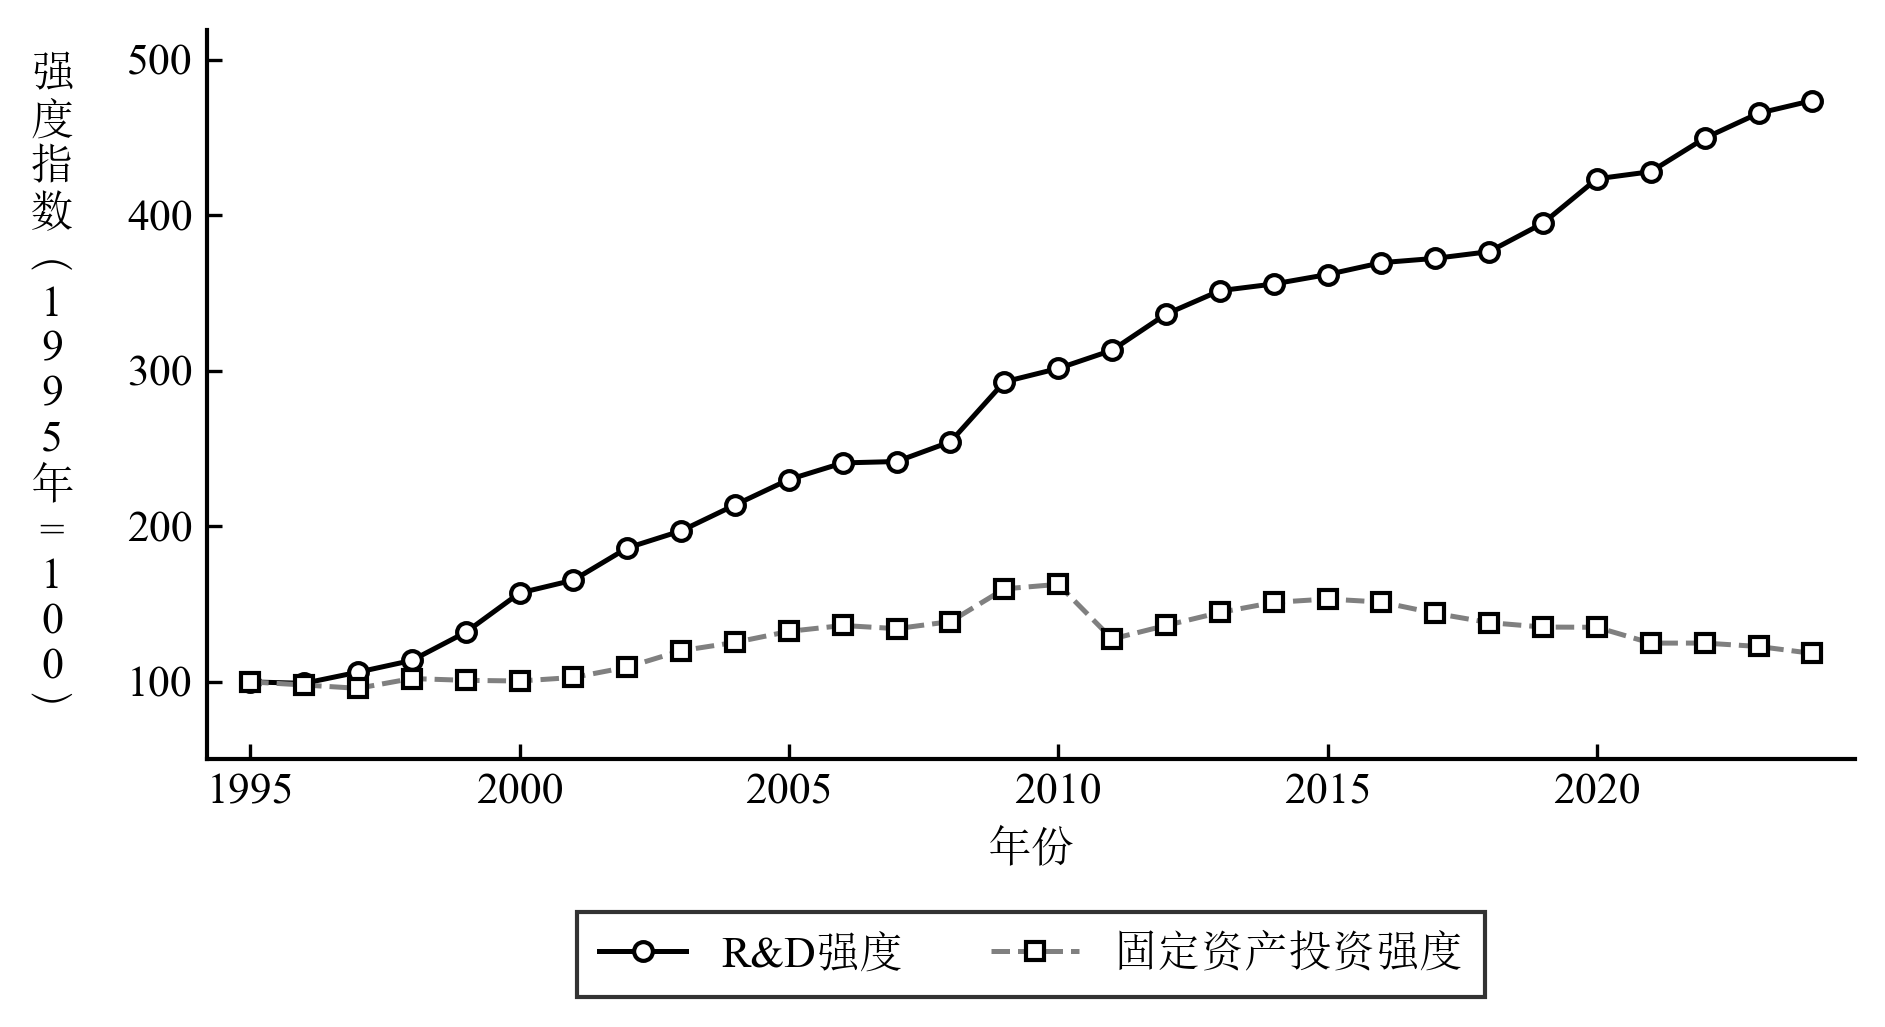
\includegraphics[width=0.78\linewidth,height=0.62\textheight,keepaspectratio]{figures/paper/macro-rd-fai-1995.png}
    \caption{1995--2023 年研发支出指数与固定资产投资指数（1995 年=100）}
  \end{figure}
\end{frame}

\begin{frame}{这个图告诉了我们什么？}
  大家看一下这张图，两条线的走势一目了然：

  \begin{itemize}
    \item 1995 年的时候，中国研发经费占全社会固定资产投资的比重，\textbf{不到 2\%}；
    \item 到了 2023 年，这个数字已经超过了 \textbf{10\%}；
    \item 而且大家注意，两条线的分化在 2008 年金融危机之后明显加速了。
  \end{itemize}

  \vspace{0.5em}
  换句话说，中国企业的投资正在发生一个结构性的转变：\textbf{盖厂房、买设备的钱相对变少了，搞研发、做创新的钱相对变多了}。
\end{frame}

\begin{frame}{已有解释，以及它们没有回答的问题}
  怎么理解这个趋势？已有的研究大致给了两种说法：

  \begin{itemize}
    \item 一种比较悲观：实物投资收缩说明企业信心不足、总需求疲软，担心是不是资产负债表衰退；
    \item 另一种相对乐观：软件、数据、专利这些无形资产正在替代传统的机器设备。
  \end{itemize}

  \vspace{0.5em}
  但我总觉得这两种解释都缺了一环——

  \begin{cautionbox}{一个绕不过去的问题}
    在融资难、融资贵普遍存在的现实下，企业为什么能\emph{一边减少实物投资、一边扩大研发投入}？这种"此消彼长"如果不是简单的规模收缩，那背后的驱动力是什么？
  \end{cautionbox}
\end{frame}

\begin{frame}{为什么说这是一个可识别的问题？}
  \begin{itemize}
    \item 我们注意到，这个投资结构转变的时间窗口，恰好与中国产业数字化政策的推进节奏高度吻合。
    \item 尤其是\emph{两化融合管理体系贯标}——这是一个企业层面的数字化治理能力认证，截至 2025 年 4 月，贯标企业已经超过 \textbf{7.4 万家}。
    \item 对我们做实证的人来说，这个制度设计提供了一个很好的识别条件：\emph{认证通过日可观测，试点分批推进}——天然就是一个交叠 DID 的设定。
  \end{itemize}

  \begin{findingbox}{所以本文要回答的核心问题是}
    数字化通过什么样的渠道，让原本受融资约束压制的企业，把资金从低效的实物囤积转向了研发和创新？
  \end{findingbox}
\end{frame}

\begin{frame}{切入的角度：从融资契约看问题}
  我们的分析角度可能和已有文献不太一样——我们是从\emph{融资契约是怎么写的}这个角度切入的。

  \begin{itemize}
    \item 在金融市场不完美的情况下，企业借钱很大程度上要靠资产做抵押。
    \item 这就导致实物资产（厂房、设备、土地）在企业账上\emph{同时承担两种角色}：既是干活的工具，也是借钱的凭据。
    \item 当"借钱的凭据"这个角色压倒"干活的工具"时，企业就会把实物资本推到超出生产需要的水平——我们管这叫\emph{抵押囤积}。
  \end{itemize}
\end{frame}

\begin{frame}{数字化的关键作用：让信息替代抵押}
  那数字化在其中扮演什么角色？这里需要引入近年文献的一个重要发现：

  \begin{itemize}
    \item Lian 和 Ma（2021）发现，美国大约 \textbf{80\%} 的企业债务其实不是靠资产抵押，而是基于经营现金流；
    \item 万晓莉等（2025）进一步记录了中国企业的融资模式也在从抵押物导向转向现金流导向。
  \end{itemize}

  \vspace{0.4em}
  这意味着什么？意味着企业借钱其实有两条路——\emph{资产抵押}和\emph{现金流抵押}。

  \begin{findingbox}{数字化的角色：信息替代抵押}
    数字化让企业的经营活动变得更加标准化、可记录、可验证。当银行能看到、能相信企业的经营数据时，现金流信息就开始替代实物抵押品发挥作用。这时候，那些原本为了借钱而多囤的设备厂房，就可以慢慢退出了。
  \end{findingbox}
\end{frame}

\begin{frame}{本文的三个边际贡献}
  \begin{enumerate}
    \item \textbf{理论上}：我们把资产抵押和现金流抵押同时放进一个两期投融资模型，推导出一个关于实物资本边际收益的\emph{门槛命题}——这解释了为什么同样面临数字化，不同企业的投资调整方向可能截然不同。
    \item \textbf{识别上}：利用两化融合贯标的分批推进构造准自然实验，并吸收了 Nagengast 和 Yotov（2025）、Bertolotti（2026）处理预期效应的最新方法。
    \item \textbf{机制上}：沿着\emph{信息替代抵押 $\rightarrow$ 抵押囤积出清 $\rightarrow$ 配置效率改善}这条逻辑链，给出了层层递进的经验证据。
  \end{enumerate}
\end{frame}
